\documentclass{article}

\usepackage{graphicx}
\usepackage{tikz}
\usepackage{tikzsymbols}
\usetikzlibrary{calc,patterns,shapes.geometric}
\pagestyle{empty}
\usepackage[margin=0pt]{geometry}
\geometry{papersize={14in,12in}}

\def\centerarc[#1](#2)(#3:#4:#5){\draw[#1] ($(#2)+({#5*cos(#3)},{#5*sin(#3)})$) arc (#3:#4:#5);}

\begin{document}
	\begin{figure}
		\centering
		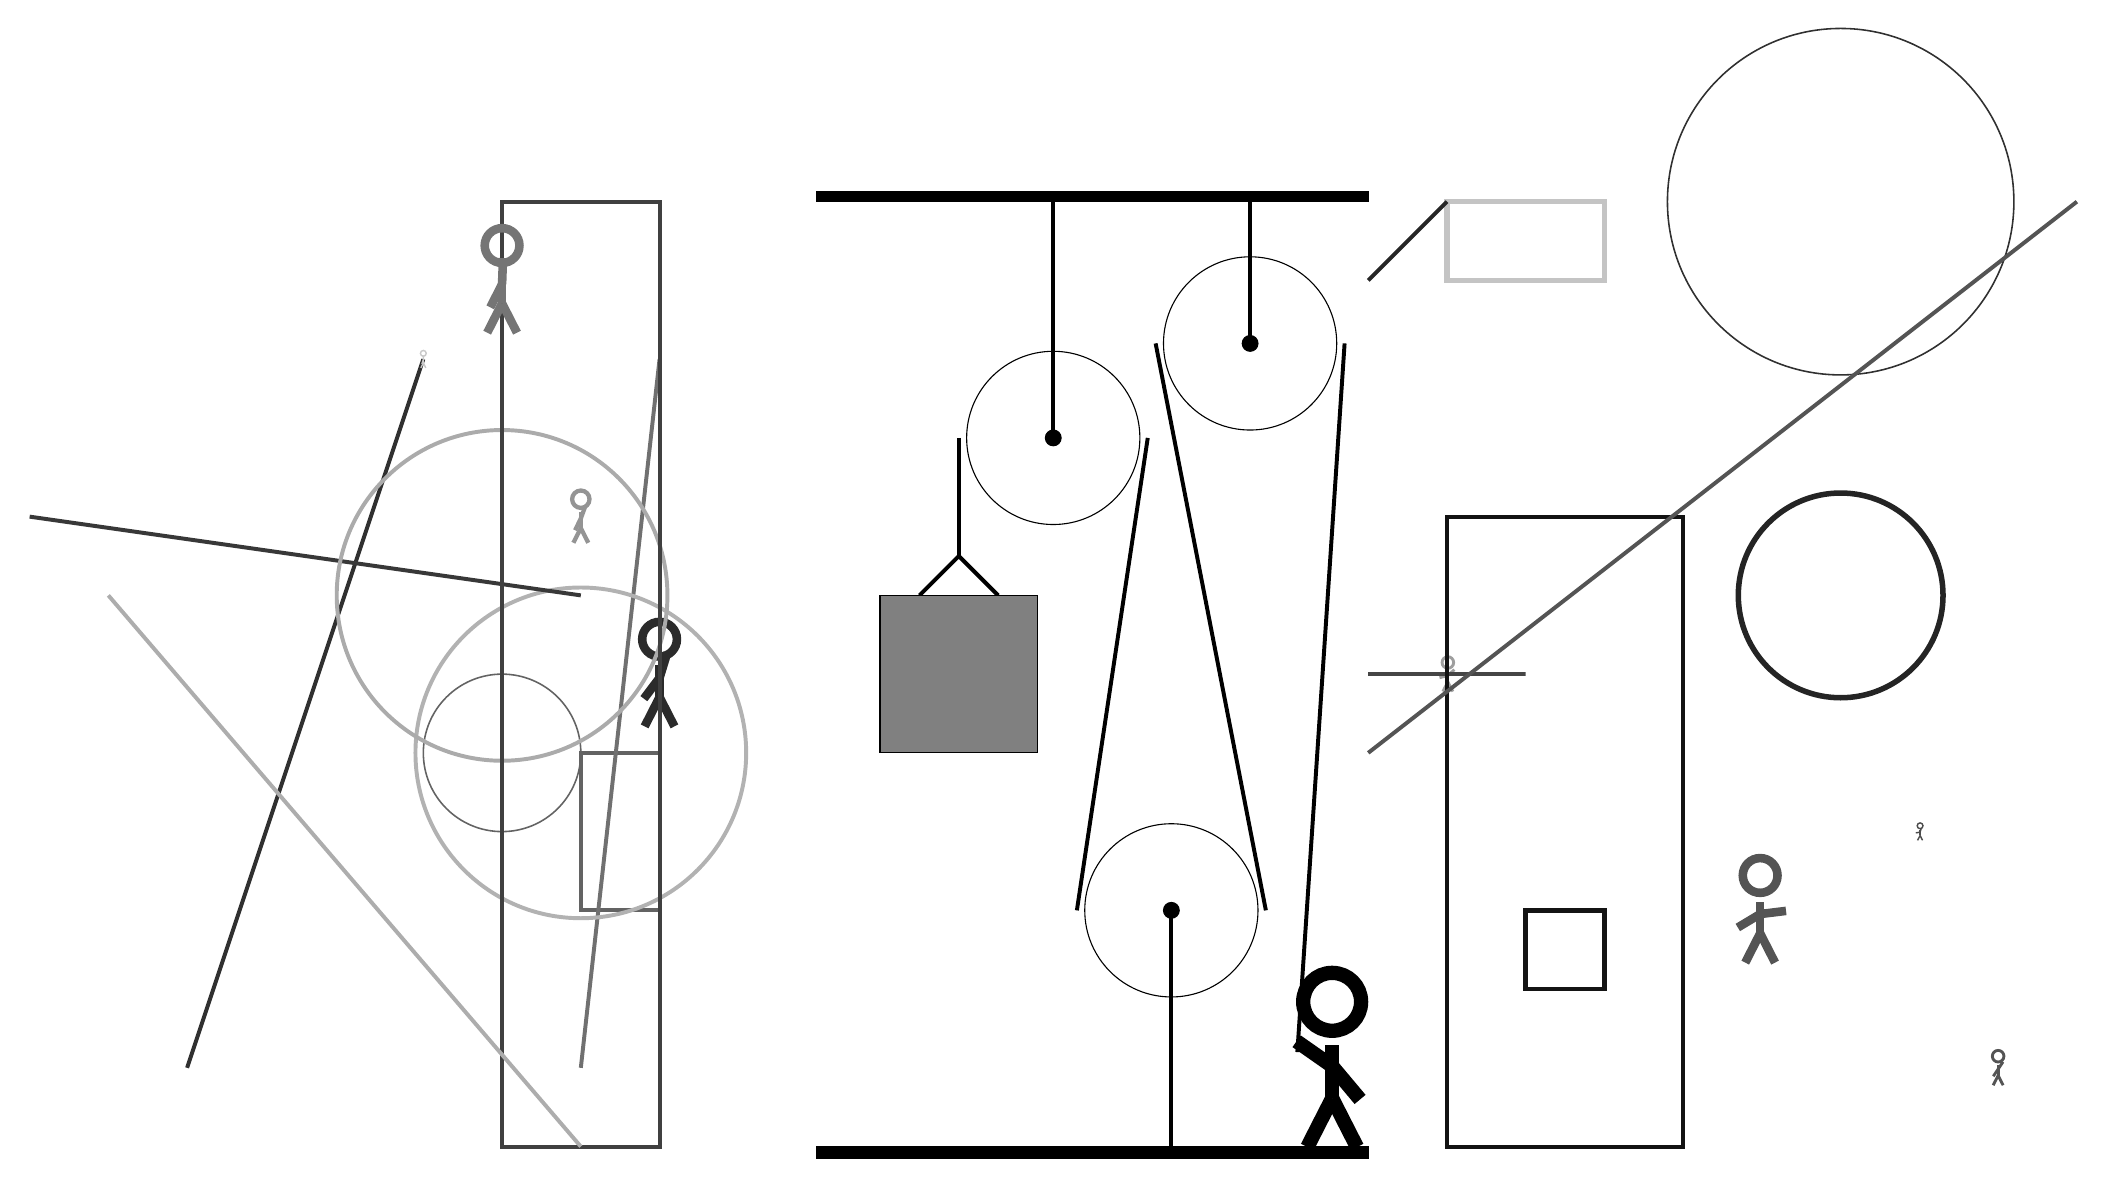
\begin{tikzpicture}
			%%%%% START %%%%%
			
			\draw[fill=black] (-2, 9) rectangle (5, 9.125);
			
			\draw (1, 6) circle (1.1);
			\draw[fill=black] (1, 6) circle (0.1);
			\draw[line width=0.5mm]  (1, 9) -- (1, 6);
			
			\draw[line width=0.2mm, color=black!18] (6, 0) rectangle (6, 3);
			
			\draw[line width=0.5mm, color=black!81](-7, 7) -- (-10, -2);
			\node[line width=0.4mm, color=black!38] at (6, 3) {\Strichmaxerl[2][16][41]};
			\draw [line width=0.7mm, color=black!86](11, 4) circle (1.3);
			\draw [line width=0.2mm, color=black!61](-6, 2) circle (1.0);
			
			\draw[line width=0.5mm, color=black!61] (-4, 2) rectangle (-5, 0);
			
			\node[line width=0.7mm, color=black!21] at (-7, 7) {\Strichmaxerl[1][70][89]};
			\draw[line width=0.6mm, color=black!92] (7, 0) rectangle (8, -1);
			\draw[line width=0.7mm, color=black!23] (6, 9) rectangle (8, 8);
			
			\draw[line width=0.5mm, color=black!56](-5, -2) -- (-4, 7);
			\draw [line width=0.5mm, color=black!30](-5, 2) circle (2.1);
			\draw [line width=0.2mm, color=black!81](11, 9) circle (2.2);
			\node[line width=0.3mm, color=black!42] at (-5, 5) {\Strichmaxerl[3][64][70]};
			\draw[line width=0.6mm, color=black!73] (5, 3) rectangle (7, 3);
			\node[line width=0.5mm, color=black!67] at (13, -2) {\Strichmaxerl[2][56][56]};
			\node[line width=0.2mm, color=black!83] at (-4, 3) {\Strichmaxerl[6][53][73]};
			\draw[line width=0.5mm, color=black!78](-5, 4) -- (-12, 5);
			
			\draw[line width=0.5mm, color=black!85](6, 9) -- (5, 8);
			\node[line width=0.7mm, color=black!67] at (10, 0) {\Strichmaxerl[6][31][7]};
			\node[line width=0.5mm, color=black!70] at (12, 1) {\Strichmaxerl[1][8][74]};
			\draw [line width=0.5mm, color=black!33](-6, 4) circle (2.1);
			
			\draw[line width=0.5mm, color=black!75] (-4, 9) rectangle (-6, -3);
			\draw[line width=0.5mm, color=black!93] (6, -3) rectangle (9, 5);
			\draw[line width=0.5mm, color=black!67](5, 2) -- (14, 9);
			\draw[line width=0.5mm, color=black!32](-5, -3) -- (-11, 4);
			
			\node[line width=0.5mm, color=black!54] at (-6, 8) {\Strichmaxerl[6][63][88]};
			
			
			\draw[fill=white](2.5, 0) circle (1.1);
			\draw[fill=black] (2.5, 0) circle (0.1);
			\draw[line width=0.5mm]  (2.5, -3) -- (2.5, 0);
			
			\draw[fill=white](3.5, 7.2) circle (1.1);
			\draw[fill=black] (3.5, 7.2) circle (0.1);
			\draw[line width=0.5mm] (3.5, 9) -- (3.5, 7.2);
			
			\draw[line width=0.5mm] (-0.7, 4.0) -- (-0.2, 4.5) -- (0.3, 4.0);
			\draw[fill=black!50] (-1.2, 4.0) rectangle (0.8, 2.0);
			
			\draw[line width=0.5mm] (-0.2, 6) -- (-0.2, 4.5);
			\centerarc[line width=0.5mm](1, 6)(0:180:1.2000000000000002);
			\draw[line width=0.5mm](2.2, 6) -- (1.3, 0);
			\centerarc[line width=0.5mm](2.5, 0)(180:360:1.2000000000000002);
			\draw[line width=0.5mm](3.7, 0) -- (2.3, 7.2);
			\centerarc[line width=0.5mm](3.5, 7.2)(0:180:1.2000000000000002);
			\draw[line width=0.5mm](4.7, 7.2) -- (4.1, -1.8);
			
			\node at (4.5, -1.9) {\Strichmaxerl[10][-35][-50]};
			
			\draw[fill=black] (-2, -3) rectangle (5, -3.15);
			
			%%%%% END %%%%%
		\end{tikzpicture}
	\end{figure}	
\end{document}